\documentclass[12pt,hyperref,a4paper,UTF8]{ctexart}
\usepackage{HDUReport}
\usepackage{listings}
\usepackage{xcolor}
\usepackage{graphicx}
\usepackage{setspace}
\usepackage{float}
\setstretch{1.5} % 设置全局行距为1.5倍

\usepackage{enumitem} % 载入enumitem包以便自定义列表环境
\setlist[itemize]{itemsep=0pt, parsep=0pt} % 设置itemize环境的项目间距和段落间距

\setmainfont{Times New Roman} % 英文正文为Times New Roman


\usepackage{tikz}
\usetikzlibrary{shapes.geometric, arrows}
\usetikzlibrary{positioning, arrows.meta}
\usetikzlibrary{calc}
%封面页设置
{   
    %标题
    \title{ 
        \vspace{1cm}
        \heiti \Huge \textbf{《单片机原理及应用》作业报告} \par
        \vspace{1cm} 
        \heiti \Large {\underline{实验报告3第三部分:频率与占空比调节}   } 
        \vspace{3cm}
    
    }

    \author{
        \vspace{0.5cm}
        \kaishu\Large 学院\ \dlmu[9cm]{卓越学院} \\ %学院
        \vspace{0.5cm}
        \kaishu\Large 学号\ \dlmu[9cm]{23040447} \\ %班级
        \vspace{0.5cm}
        \kaishu\Large 姓名\ \dlmu[9cm]{陈文轩} \qquad  \\ %学号
        \vspace{0.5cm}
        \kaishu\Large 专业\ \dlmu[9cm]{智能硬件与系统(电子信息工程)} \qquad \\ %姓名 
    }
        
    \date{\today} % 默认为今天的日期,可以注释掉不显示日期
}
%%------------------------document环境开始------------------------%%
\begin{document}

%%-----------------------封面--------------------%%
\cover
\thispagestyle{empty} % 首页不显示页码
%%------------------摘要-------------%%
%\newpage
%\begin{abstract}




%\end{abstract}

%\thispagestyle{empty} % 首页不显示页码

%%--------------------------目录页------------------------%%
% \newpage
% \tableofcontents
% \thispagestyle{empty} % 目录不显示页码

%%------------------------正文页从这里开始-------------------%
\newpage
\setcounter{page}{1} % 让页码从正文开始编号

%%可选择这里也放一个标题
%\begin{center}
%    \title{ \Huge \textbf{{标题}}}
%\end{center}


\textbf{原题目:设计一个简易方波波形发生器,在按键K1(接INT0脚)的触发下可实现1KHz,100Hz,10Hz,1Hz的波形切换。用C语言编程。(选做:若按键K2(接INT1)实现当前频率波形下的占空比可调,如何实现?)}


\section{实验代码}

\begin{lstlisting}[language=C, caption={实验程序}]
#include <reg51.h>

// 宏定义
#define FOSC 12000000       // 晶振频率 12MHz
#define TIMER_RELOAD_1KHZ (65536 - FOSC / 12 / 2 / 1000 /2) // 1KHz定时器初值 因为是半周期
#define TIMER_RELOAD_100HZ (65536 - FOSC / 12 / 2 / 100 /2) // 100Hz定时器初值
#define TIMER_RELOAD_10HZ (65536 - FOSC / 12 / 2 / 10 /2)   // 10Hz定时器初值
//#define TIMER_RELOAD_1HZ (65536 - FOSC / 12 / 2 / 1 /2)     // 1Hz定时器初值 250,000超出范围了
//因为是半周期翻转电平 所以再乘以2补偿
sbit P2_0 = P2^0; // 方波输出引脚
unsigned char mode = 0; // 模式切换变量

// 外部中断1服务函数
void INT0_ISR(void) interrupt 0 {
    mode = (mode + 1) % 4; // 模式循环切换
}

// 定时器0中断服务函数
void Timer0_ISR(void) interrupt 1 {
        static int counter_1HZ=0; //基于10HZ的分频,计数十次就是1HZ
    TH0 = (mode == 0) ? (TIMER_RELOAD_1KHZ >> 8) :
            (mode == 1) ? (TIMER_RELOAD_100HZ >> 8) :
            (mode == 2) ? (TIMER_RELOAD_10HZ >> 8) :
                        (TIMER_RELOAD_10HZ >> 8);
    TL0 = (mode == 0) ? (TIMER_RELOAD_1KHZ & 0xFF) :
            (mode == 1) ? (TIMER_RELOAD_100HZ & 0xFF) :
            (mode == 2) ? (TIMER_RELOAD_10HZ & 0xFF) :
                        (TIMER_RELOAD_10HZ & 0xFF);
    
        if (mode==3) //1HZ
        {
            counter_1HZ++;
            if (counter_1HZ==10)
            {
                counter_1HZ=0;
                P2_0 = ~P2_0;
                
            }
        }
        else
        {
            P2_0 = ~P2_0; // 其他模式,直接翻转P2.0引脚电平
        }
    
}

void main() {
    // 初始化外部中断1
    IT0 = 1;  // 下降沿触发
    EX0 = 1;  // 使能外部中断0
    EA = 1;   // 开启总中断

    // 初始化定时器0
    TMOD = 0x01; // 定时器0,模式1(16位定时)
    TH0 = TIMER_RELOAD_1KHZ >> 8;
    TL0 = TIMER_RELOAD_1KHZ & 0xFF;
    ET0 = 1; // 使能定时器0中断
    TR0 = 1; // 启动定时器0

    P2_0 = 0; // 初始化P2.0为低电平

    while (1) {
        // 主循环,所有逻辑在中断中处理
    }
}
   
    
\end{lstlisting}

\section{实验效果}

\begin{figure}[H] % [H] 表示强制当前位置插入
    \centering
    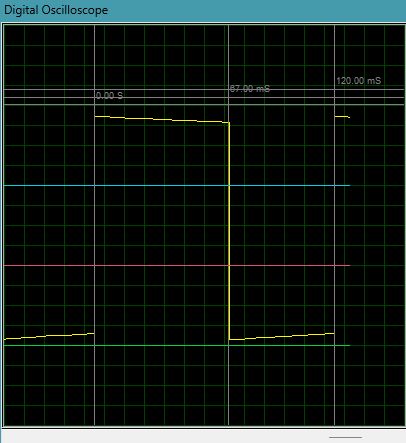
\includegraphics[width=1\textwidth]{figures/201.png} % 调整宽度为文本宽度的 80%
    \caption{Proteus示波器效果,周期手动测量120ms,高电平67ms,占空比55.8\% } %图片标题
    \label{fig:example} % 图片标签,用于引用
\end{figure}






\section{流程图}

\begin{figure}[H]
    \centering
    \begin{tikzpicture}[
        node distance=0.7cm, % 进一步缩小节点间距
        startstop/.style={rectangle, rounded corners, minimum width=1.8cm, minimum height=0.5cm, text centered, draw=black, fill=red!30},
        process/.style={rectangle, minimum width=1.8cm, minimum height=0.5cm, text centered, draw=black, fill=blue!30},
        decision/.style={diamond, aspect=2, minimum width=1.8cm, minimum height=0.6cm, text centered, draw=black, fill=green!30},
        arrow/.style={thick, -Stealth}
    ]

        % ===== 主流程 =====
        \node (start) [startstop] {程序开始};
        \node (initVars) [process, below=of start] {初始化变量};
        \node (initTimer) [process, below=of initVars] {初始化定时器};
        \node (setHigh) [process, below=of initTimer] {设置P2.0为高电平};
        \node (mainLoop) [process, below=of setHigh] {主循环等待中断};

        % ===== 中断处理 =====
        \node (interrupt) [decision, right=2.5cm of mainLoop] {定时器中断触发?};
        \node (counterInc) [process, below=0.8cm of interrupt] {计数器+1};
        \node (highCheck) [decision, below=0.8cm of counterInc] {P2.0为高电平?};
        \node (lowCheck) [decision, right=2.5cm of highCheck] {P2.0为低电平?};
        \node (setLow) [process, below=0.8cm of highCheck] {设置P2.0为低电平};
        \node (setHighAgain) [process, below=0.8cm of lowCheck] {设置P2.0为高电平};
        \node (resetCounter) [process, below=0.8cm of setLow, xshift=1.5cm] {计数器清零};

        % ===== 箭头连接 =====
        % 主流程
        \draw [arrow] (start) -- (initVars);
        \draw [arrow] (initVars) -- (initTimer);
        \draw [arrow] (initTimer) -- (setHigh);
        \draw [arrow] (setHigh) -- (mainLoop);

        % 中断处理
        \draw [arrow] (mainLoop.east) -- ++(1cm,0) |- (interrupt.west);
        \draw [arrow] (interrupt.south) -- node[right] {是} (counterInc.north);
        \draw [arrow] (counterInc.south) -- (highCheck.north);
        \draw [arrow] (highCheck.east) -- node[above] {否} (lowCheck.west);
        \draw [arrow] (lowCheck.south) -- node[right] {是} (setHighAgain.north);
        \draw [arrow] (setHighAgain.south) -- ++(0,-0.4cm) -| (resetCounter.east);
        \draw [arrow] (highCheck.south) -- node[right] {是} (setLow.north);
        \draw [arrow] (setLow.south) -- ++(0,-0.4cm) -| (resetCounter.west);

        % 返回主循环
        \draw [arrow] (resetCounter.north) -- ++(0,0.4cm) -| (mainLoop.south);

        % 中断否路径
        \draw [arrow] (interrupt.east) -- ++(1cm,0) |- ++(0,-3.5cm) -| (mainLoop.east);

    \end{tikzpicture}
    \caption{程序流程图}
    \label{fig:program_flowchart}
\end{figure}




\section{实验体会}


通过本次实验,我掌握了定时器T1的方式2配置及中断机制的应用,成功实现了周期为120ms、占空比为57\%的波形输出。实验中,通过0.5ms定时中断累加解决了定时器溢出时间不足的问题,并通过宏定义灵活计算占空比,提升了代码的通用性。Proteus仿真验证了波形输出的正确性,进一步加深了对定时器和中断机制的理解,为后续单片机开发奠定了基础。




\end{document}